\documentclass[a4paper,12pt]{article}
\usepackage{amsmath, amssymb}
\usepackage{xcolor}
\usepackage[most]{tcolorbox}
\usepackage{multicol}
\usepackage{geometry}
\usepackage{enumitem}
\usepackage{tasks}  % pour lister des items en colonnes
\usepackage{yhmath}
\usepackage{graphicx}% pour \includegraphics
\usepackage{tikz}
\usetikzlibrary{calc,angles,quotes}
% Définition de la "pic" "tick"
\tikzset{
  pics/tick/.style args={#1}{
    code={
      % "#1" correspond à la longueur du tick.
      \draw[line width=1pt, line cap=round] (-#1/2,0) -- (#1/2,0);
    }
  }
}

\graphicspath{ {../Images/} } % chemin vers le dossier d'images
\hyphenpenalty=1000

\geometry{left=1.5cm, right=1.5cm, top=2cm, bottom=2cm}

\tcbuselibrary{theorems}

\definecolor{PurpleEx}{HTML}{5d478b}
\definecolor{GrayEx}{HTML}{f2f2f2}
\definecolor{GrayBG}{HTML}{d9d9d9}
\definecolor{BlackSav}{HTML}{000000}
\definecolor{RedMet}{HTML}{cd5556}

\title{
  \centering
  \tcbset{colframe=BlackSav,colback=GrayBG}
  \tcbox[tikznode]{
    Chapitre 7 \\Produit scalaire
  }
}
\author{}
\date{}

\newtcbtheorem
[]% init options
{exercice}% name
{Exercice}% title
{%
  colback=GrayEx,
  colframe=PurpleEx,
  fonttitle=\bfseries,
  breakable=true
}% options
{ex}% prefix

\newtcbtheorem
[]% init options
{method}% name
{Méthode}% title
{%
  theorem name,
  colback=GrayBG,
  colframe=RedMet,
  fonttitle=\bfseries,
}% options
{met}% prefix

\begin{document}

\maketitle

\begin{multicols}{2}

  \begin{exercice}[title=Exercice 1 $\star$ { [Calculer] }]{}{}
    On considère deux vecteurs \(\vec{u}\) et \(\vec{v}\) tels que \(\|\vec{u}\| = 2\), \(\|\vec{v}\| = 3\) et \(\|\vec{u} + \vec{v}\| = 4\).
    Les vecteurs \(\vec{u}\) et \(\vec{v}\) sont-ils orthogonaux ?
  \end{exercice}

  \begin{exercice}[title=Exercice 2 $\star$ { [Représenter] }]{}{}
    Soit \(ABCD\) un carré de centre \(O\).
    En utilisant uniquement les points \(A\), \(B\), \(C\), \(D\) et \(O\), citer cinq produits scalaires nuls.
  \end{exercice}

  \begin{exercice}[title=Exercice 3 $\star$ { [Calculer, Représenter] }]{}{}
    Dans chaque cas, déterminer \(\overrightarrow{AB} \cdot \overrightarrow{BC}\).
    \begin{enumerate}
      \item \(\mathrm{AB} = 2,\quad \mathrm{AC} = 2,\quad \mathrm{BC} = 1.\)
      \item \(\mathrm{AB} = \sqrt{3},\quad \mathrm{AC} = \sqrt{5},\quad \mathrm{BC} = \sqrt{7}.\)
    \end{enumerate}
  \end{exercice}

  \begin{exercice}[title=Exercice 4 $\star$ { [Raisonner] }]{}{}
    Soient \(\vec{u}\) et \(\vec{v}\) deux vecteurs. On considère la proposition suivante :
    \[
      \text{« Si } \vec{u} \cdot \vec{v} = 0,\text{ alors } \vec{u} = \vec{0} \text{ ou } \vec{v} = \vec{0}\text{. »}
    \]
    \begin{enumerate}
      \item La proposition est-elle vraie ?
      \item La réciproque de cette proposition est-elle vraie ou fausse ?
    \end{enumerate}
  \end{exercice}

  \begin{exercice}[title=Exercice 5 $\star$ { [Calculer] }]{}{}
    Dans un repère orthonormé \(\bigl(O;\,\vec{i},\,\vec{j}\bigr)\), on considère deux vecteurs
    \[
      \vec{u}\binom{3}{2}
      \quad\text{et}\quad
      \vec{v}\binom{6}{-4}
    \]
    \begin{enumerate}
      \item Calculer \(\|\vec{u}\|\), \(\|\vec{v}\|\) et \(\|\vec{u} + \vec{v}\|\).
      \item Calculer \(\vec{u}\cdot\vec{v}\) à partir de la définition du produit scalaire. Que peut-on dire sur les vecteurs \(\vec{u}\) et \(\vec{v}\) ?
      \item Retrouver le résultat précédent à l'aide de la formule du produit scalaire avec les coordonnées.
    \end{enumerate}
  \end{exercice}

  \begin{exercice}[title=Exercice 6 $\star$ { [Calculer] }]{}{}
    Dans chaque cas, on donne les coordonnées de quatre points \(A,\ B,\ C\) et \(D\) dans un repère orthonormé. Calculer \(\overrightarrow{AB} \cdot \overrightarrow{CD}\).
    \begin{enumerate}
      \item
        \(A(0\,;\,5),\quad B(-7\,;\,8),\\ C(1\,;\,5),\quad D(-3\,;\,4)\).
      \item
        \(A(\sqrt{2}\,;\,1),\quad B(4\,;\,\sqrt{3}),\\ C(1\,;\,2),\quad D(-2\,;\,-\tfrac{1}{2})\).
    \end{enumerate}
  \end{exercice}

  \begin{exercice}[title=Exercice 7 $\star\star$ { [Chercher, Calculer] }]{}{}
    Dans un repère orthonormé, on considère les six points
    $A(1\,;\,1)$, $B(4\,;\,0)$, $C(9\,;\,10)$, $D(-2\,;\,3)$ et $E(-1\,;\,-2)$.
    \begin{enumerate}
      \item Placer les points dans un repère puis conjecturer quelles sont les droites perpendiculaires et les droites parallèles parmi les droites \((AD)\), \((BC)\) et \((AE)\).
      \item Démontrer cette conjecture.
    \end{enumerate}
  \end{exercice}

  \begin{exercice}[title=Exercice 8 $\star\star$ { [Calculer] }]{}{}
    Soient \(\vec{u}\) et \(\vec{v}\) deux vecteurs tels que \\
    \(\|\vec{u}\| = 3\), \(\|\vec{v}\| = 2\) et \(\vec{u}\cdot\vec{v} = 1\).
    Calculer :
    \[
      \vec{v}\cdot\vec{u},
      \quad 7\,\vec{u}\cdot\vec{v},
      \quad (\vec{u} - \vec{v})^2,
      \quad (\vec{u} + \vec{v})\cdot(\vec{u} - \vec{v}).
    \]
  \end{exercice}

  \begin{exercice}[title=Exercice 9 $\star\star$ { [Calculer] }]{}{}
    Soient \(\vec{u}\) et \(\vec{v}\) deux vecteurs orthogonaux. Simplifier au maximum les expressions suivantes :
    \begin{tasks}[style=itemize](1)
      \task \(\bigl(2\,\vec{u}\bigr)\cdot\bigl(5\,\vec{v}\bigr)\)
      \task \(\vec{u}\cdot\bigl(\vec{u} - \vec{v}\bigr)\)
      \task \(\bigl(\vec{u} + \vec{v}\bigr)^2\)
    \end{tasks}
  \end{exercice}

  \begin{exercice}[title=Exercice 10 $\star\star$ { [Raisonner] }]{}{}
    Pour chaque proposition, dire si elle est vraie ou fausse en justifiant :
    \begin{enumerate}
      \item Pour tous points \(A,\ B,\ C\) et \(D\), on a \(\overrightarrow{AB}\cdot\overrightarrow{CD} = -\,\overrightarrow{AB}\cdot\overrightarrow{DC}\).
      \item Il existe des points \(A,\ B,\ C\) et \(D\) tels que \(\overrightarrow{AB}\cdot\overrightarrow{CD} = -\,\overrightarrow{AB}\cdot\overrightarrow{DC}\).
      \item Pour tous points \(A,\ B,\ C\) et \(D\), \(\overrightarrow{AB}\cdot\overrightarrow{CD} = \overrightarrow{BA}\cdot\overrightarrow{DC}\).
      \item Il existe des points \(A,\ B,\ C\) et \(D\) tels que \(\overrightarrow{AB}\cdot\overrightarrow{CD} = -\,\overrightarrow{BA}\cdot\overrightarrow{DC}\).
      \item Soient \(A,\ B,\ C\) et \(D,\ E\) cinq points. Les points \(D\) et \(E\) sont confondus si, et seulement si, \(\overrightarrow{AB}\cdot\overrightarrow{CD} = \overrightarrow{AB}\cdot\overrightarrow{CE}\).
    \end{enumerate}
  \end{exercice}

  \begin{exercice}[title=Exercice 11 $\star$ { [Calculer] }]{}{}
    \begin{enumerate}
      \item Soient \(A,\ B\) et \(C\) trois points tels que \(\mathrm{AB} = 1\), \(\mathrm{AC} = 5\) et \(\bigl(\overrightarrow{AB}, \overrightarrow{AC}\bigr) = -\dfrac{\pi}{4}\).
        Déterminer \(\overrightarrow{AB}\cdot\overrightarrow{AC}\).
      \item Soient \(A,\ B\) et \(C\) tels que \(\mathrm{AB} = 4\), \(\mathrm{AC} = 5\) et \(\overrightarrow{AB}\cdot\overrightarrow{AC} = 10\).\\
        Déterminer la valeur de l'angle \(\bigl(\overrightarrow{AB}, \overrightarrow{AC}\bigr)\) en supposant qu'il appartient à l'intervalle \([0;\;\pi]\).
    \end{enumerate}
  \end{exercice}

  \begin{exercice}[title=Exercice 12 $\star$ { [Représenter, Calculer] }]{}{}
    Soit \(H\) le projeté orthogonal de \(C\) sur \(\bigl(AB\bigr)\).\\
    Dans chaque cas, déterminer \(\overrightarrow{AB}\cdot\overrightarrow{AC}\).
    \begin{enumerate}
      \item \(\mathrm{AB} = 5,\quad \mathrm{AH} = 6\) et \(H \in \bigl[AB\bigr)\).
      \item \(\mathrm{AB} = 2,\quad \mathrm{AH} = \dfrac{1}{3}\) et \(H \notin \bigl[AB\bigr)\).
    \end{enumerate}
  \end{exercice}

  \begin{exercice}[title=Exercice 13 $\star\star$ { [Représenter, Calculer] }]{}{}
    Pour chacune des figures ci-dessous, calculer en justifiant la valeur exacte du produit scalaire
    \(
      \overrightarrow{AB} \cdot \overrightarrow{AC}.
    \)

    \begin{enumerate}
      \item\ \linebreak
        \vspace{-2em}
        \begin{center}
          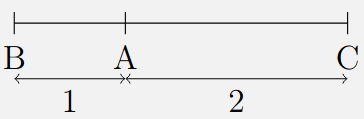
\includegraphics[width=0.7\linewidth]{swappy-20250226_144649.png}
        \end{center}

      \item\ \linebreak
        \vspace{-2em}
        \begin{center}
          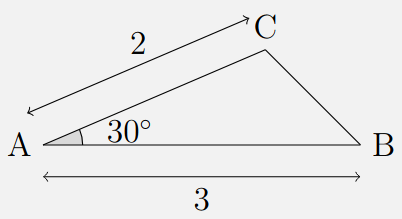
\includegraphics[width=0.7\linewidth]{swappy-20250226_144717.png}
        \end{center}

      \item\ \linebreak
        \vspace{-2em}
        \begin{center}
          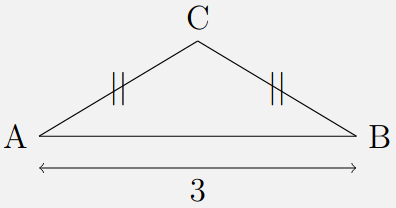
\includegraphics[width=0.7\linewidth]{swappy-20250226_144732.png}
        \end{center}

      \item\ \linebreak
        \vspace{-2em}
        \begin{center}
          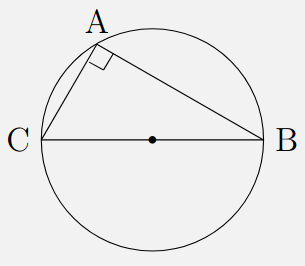
\includegraphics[width=0.55\linewidth]{swappy-20250226_144745.png}
        \end{center}

      \item\ \linebreak
        \vspace{-2em}
        \begin{center}
          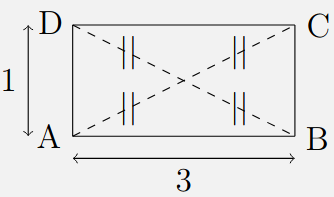
\includegraphics[width=0.6\linewidth]{swappy-20250226_144808.png}
        \end{center}

      \item\ \linebreak
        \vspace{-2em}
        \begin{center}
          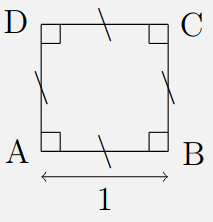
\includegraphics[width=0.4\linewidth]{swappy-20250226_144828.png}
        \end{center}

      \item\ \linebreak
        \vspace{-2em}
        \begin{center}
          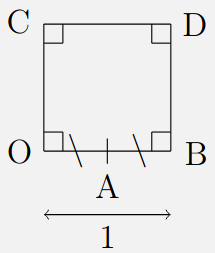
\includegraphics[width=0.4\linewidth]{swappy-20250226_144843.png}
        \end{center}

      \item\ \linebreak
        \vspace{-2em}
        \begin{center}
          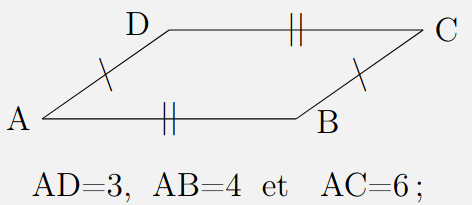
\includegraphics[width=0.85\linewidth]{swappy-20250226_144856.png}
        \end{center}

    \end{enumerate}

  \end{exercice}

  \begin{exercice}[title=Exercice 14 $\star\star$ { [Représenter, Calculer] }]{}{}
    Soit \(ABC\) un triangle tel que \(\mathrm{AB} = 7\), \(\mathrm{AC} = 6\) et \(\mathrm{BC} = 4\).
    À l'aide de la calculatrice, déterminer une mesure des trois angles du triangle en degrés (on arrondira les résultats à \(0{,}1^\circ\) près).
  \end{exercice}

  \begin{exercice}[title=Exercice 15 $\star\star\star$ { [Chercher, Représenter] }]{}{}
    Soit \(ABC\) un triangle rectangle isocèle en \(A\). On note \(I\) le milieu de \([AB]\), \(J\) le milieu de \([AC]\) et \(K\) le milieu de \([CI]\).
    Démontrer que les droites \((AK)\) et \((BJ)\) sont perpendiculaires.
  \end{exercice}

  \newcolumn

  \begin{exercice}[title=Exercice 16 $\star\star\star$ { [Chercher, Raisonner, Représenter] }]{}{}
    \begin{enumerate}
      \item Montrer que pour tous points \(A,\,B,\,C\) et \(D\) du plan,
        \[
          \overrightarrow{AB}\cdot\overrightarrow{CD}
          \;+\;
          \overrightarrow{AC}\cdot\overrightarrow{DB}
          \;+\;
          \overrightarrow{AD}\cdot\overrightarrow{BC}
          \;=\;
          0.
        \]

      \item L'objectif de cette question est de montrer que les hauteurs d'un triangle sont toujours concourantes.
        \begin{enumerate}
          \item[(a)] Soit \(ABC\) un triangle quelconque. On note \(H\) l'intersection entre la hauteur issue de \(B\) et la hauteur issue de \(C\).
            En utilisant la question 1, montrer que \((AH)\) et \((BC)\) sont perpendiculaires.
          \item[(b)] En déduire que les trois hauteurs de \(ABC\) sont concourantes en \(H\).
            \textit{Remarque :} le point d'intersection des hauteurs est appelé \textbf{orthocentre} du triangle.
        \end{enumerate}

      \item Dans un repère orthonormé, on considère le triangle \(ABC\) tel que \(A(1\,;\,-2)\), \(B(4\,;\,3)\) et \(C(-2\,;\,1)\).
        Déterminer les coordonnées de l'orthocentre du triangle \(ABC\).
    \end{enumerate}
  \end{exercice}

  \newpage

  \begin{exercice}[title=Exercice 17 $\star\star\star$ { [Modéliser, Calculer] }]{}{}
    On dispose d'une planche de \(1\,\text{m}\) de long et d'une bille de masse \(m = 100\,\text{g}\).
    À l'aide d'une cale de \(20\,\text{cm}\), on place la planche de manière à former un plan incliné comme sur la figure ci-dessous.
    \begin{center}
      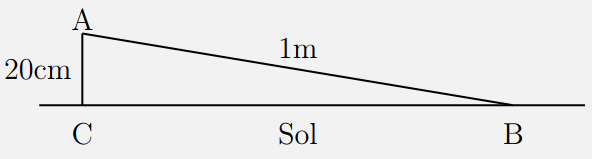
\includegraphics[width=1\linewidth]{ex17.png}
    \end{center}

    On lâche la bille depuis le point \(A\) et on la laisse rouler sur le plan incliné. On néglige les forces de frottements et on rappelle que si \(\vec{j}\) est le vecteur vertical, dirigé vers le haut et de norme \(1\), le poids de la bille est \(\vec{P} = -\,m\,g\,\vec{j}\) avec \(g = 9{,}8\,\text{m}\cdot\text{s}^{-2}\).

    Le travail du poids de la bille sur le trajet \([AB]\) est défini, en Joule, par la formule suivante :
    \[
      W \;=\; \vec{P}\,\cdot\,\overrightarrow{AB}.
    \]

    \begin{enumerate}
      \item Déterminer le travail du poids de la bille sur le trajet \([AB]\).
      \item On admet que \(W = \tfrac{1}{2}\,m\,v^2\), où \(v\) est la vitesse de la bille en arrivant au sol (au point \(B\)). Calculer \(v\).
      \item On dispose d'une autre planche de \(2\,\text{m}\) de long.
        Si on forme un plan incliné avec la même cale de \(20\,\text{cm}\), quelle sera la vitesse de la bille en arrivant au sol ? Interpréter le résultat.
    \end{enumerate}
  \end{exercice}

  \begin{exercice}[title=Exercice 18 $\star\star\star$ { [Représenter, Calculer] }]{}{}
    Si \(\vec{u}\) et \(\vec{v}\) sont deux vecteurs de l'espace, on définit le produit scalaire \(\vec{u}\cdot\vec{v}\) de la façon suivante :\\
    On considère \(O,\ A\) et \(B\) trois points tels que \(\vec{u} = \overrightarrow{OA}\) et \(\vec{v} = \overrightarrow{OB}\). On note \(\mathcal{P}\) le plan passant par les points \(O,\ A\) et \(B\) (il existe toujours). Le produit scalaire \(\vec{u}\cdot\vec{v}\) est alors égal au produit scalaire \(\overrightarrow{OA}\cdot\overrightarrow{OB}\) dans le plan \(\mathcal{P}\).

    \begin{center}
      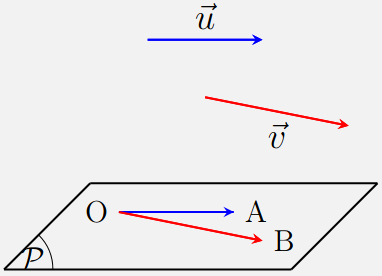
\includegraphics[width=0.8\linewidth]{ex18-1.png}
    \end{center}

    On considère un cube \(ABCDEFGH\) dont l'arête a pour longueur \(x\).

    \begin{center}
      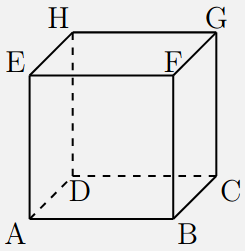
\includegraphics[width=0.45\linewidth]{ex18-2.png}
    \end{center}

    \begin{enumerate}
      \item Calculer les produits scalaires suivants en fonction de \(x\):
        \begin{enumerate}
          \item \(\overrightarrow{AB}\cdot\overrightarrow{AC}\)
          \item \(\overrightarrow{AB}\cdot\overrightarrow{AD}\)
          \item \(\overrightarrow{AH}\cdot\overrightarrow{AB}\)
          \item \(\overrightarrow{AC}\cdot\overrightarrow{AG}\)
        \end{enumerate}

      \item
        \begin{enumerate}
          \item Exprimer \(\overrightarrow{AG}\cdot\overrightarrow{BH}\) en fonction de \(x\).
          \item En déduire une mesure de l'angle \(\bigl(\overrightarrow{AG},\;\overrightarrow{BH}\bigr)\) formé par les grandes diagonales du cube.
        \end{enumerate}
    \end{enumerate}
  \end{exercice}

  \newpage


  \begin{exercice}[title=Exercice 19 $\star\star\star$ { [Représenter, Calculer] }]{}{}
    Sur le dessin ci-contre, la largeur de la cage de football est \(\mathrm{AB} = 7{,}32\,\text{m}\). Les points \(A\), \(B\) et \(D\) sont alignés. On appelle \(T\) le point où se trouve le ballon. Le triangle \(TAD\) est rectangle en \(D\). On sait par ailleurs que \(\mathrm{AD} = 9\,\text{m}\) et \(\mathrm{TD} = 18\,\text{m}\).

    \begin{enumerate}
      \item Pourquoi \(\overrightarrow{TD} \cdot \overrightarrow{DB} = 0\) ?
      \item Démontrer que \(\overrightarrow{TA} \cdot \overrightarrow{TB} = 470{,}88\).
      \item Déterminer une valeur approchée, au dixième de degré près, de l'angle de tir, c'est-à-dire de l'angle \(\widehat{ATB}\).
    \end{enumerate}
  \end{exercice}

  \newcolumn
  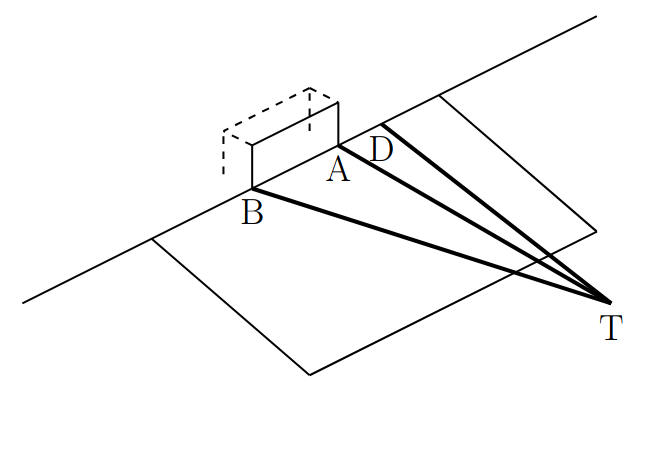
\includegraphics[width=1\linewidth]{ex19.png}

\end{multicols}

\end{document}
